\documentclass{article}
\usepackage{graphicx}
\usepackage[strings]{underscore}
\usepackage{url}
\usepackage[margin=2cm]{geometry}

\usepackage{titlesec}


\title{Fast GPU Generation of Signed Distance Fields from a Voxel Grid}
\author{Nicolas Fedor, 6683787}
\date{May 2025}

\begin{document}
\maketitle

\section{Introduction}
Voxel rendering has become an essential technique in computer graphics, enabling the representation and visualization of 3D environments through volumetric data. Unlike traditional polygon-based methods that rely on triangles and surface meshes, voxel rendering represents scenes as a grid of volumetric elements (voxels), which allows for detailed depictions of complex structures such as terrains, clouds, or medical imaging data. This approach offers several advantages, particularly in handling volumetric and procedural data, but also poses significant challenges, including high memory consumption and computational demands.

There are several differing approaches for rendering voxels, one of which is using Signed Distance Fields (SDF) and ray marching to quickly cast a ray through the voxel grid. In a typical distance field renderer mathematical functions are used to create geometry where positive values indicate distances to the nearest objects, and negative distances indicate that the ray would be within an object. In a voxel grid SDF, a 3D grid of values is used to indicate the distance to the nearest non-empty voxel that a ray could hit.

The generation of an SDF from a voxel grid can be very computationally expensive, and typical dynamic approaches are not well suited for the GPU. This paper aims to identify a fast algorithm that can make use of the GPU to quickly create voxel grid SDFs that would allow for dynamic updates to the voxel grid and see them reflected in the rendered image.

\subsection{Aims and Objectives}
The aim of this project is to develop an algorithm for generating a Signed Distance Field from voxel data; the main objectives are:

\begin{itemize}
    \item Generate a 3D texture representing the SDF of a voxel grid of the same size.
    \item Achieve an algorithm running time of under 17 milliseconds, this will allow for the use of the algorithm in a game application with a framerate of 60fps.
    \item Support dynamic updates to the voxel grid and re-generation of the SDF per the objectives above.
\end{itemize}

A voxel grid, and the associated SDF, can become very large and use a lot of memory. Optimizing the memory usage of the voxel grid and SDF will not be the focus of this paper as other methods have already been developed for the efficient compression of voxel grids.

\section{Literature Review}
This chapter will provide an overview of the existing techniques for rendering voxel data, including traditional mesh-based methods and recent advances using ray tracing and sparse voxel representations.

\subsection{Mesh-based Rendering}
Mesh-based rendering is the most common technique for representing 3D objects in computer graphics. It involves defining the surface of an object using a collection of polygons, typically triangles, which are then rendered using the GPU's rasterization pipeline. This is a well-established approach, that is the default method for rendering 3D graphics in most applications.

Volumetric voxel data can be converted to a mesh representation using techniques such as Marching Cubes~\cite{Amran_1998}, which extract the surface of the volume by sampling the voxel data; or another simpler, popular, approach is to use greedy meshing~\cite{mikolalysenko_2012}, which relies on creating a mesh by merging adjacent voxels with the same material into a single quad face in the mesh, see Figure~\ref{fig:greedy}. These approaches allow for storing voxel data uncompressed and so dynamic updates to voxel data are quick. However, the generation of the mesh becomes a bottleneck as the resolution of the voxel data increases.

\begin{figure}[thp]
    \begin{center}
        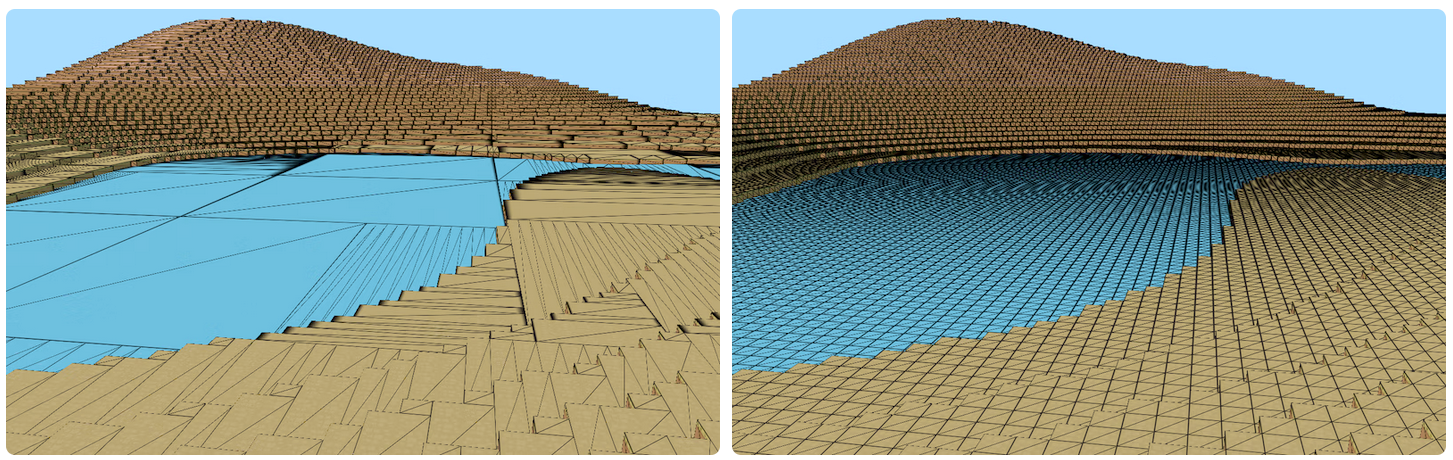
\includegraphics[width=0.8\textwidth]{figures/greedy.png}
    \end{center}
    \caption{Comparison of creating a mesh for voxel data with (left) and without (right) greedy meshing~\cite{Gedge_2014}.}
    \label{fig:greedy}
\end{figure}

\subsection{Ray Marching}
Ray marching, a specialized form of ray tracing, is another technique for rendering voxel data. It involves casting a ray through a 3D grid of voxels and sampling the voxel data along the ray to determine the color and opacity of the volume at each point. Ray marching can be implemented on the GPU using compute shaders, avoiding the creation of a mesh, instead the GPU can operate directly on the voxel data, which can be stored in a compressed format.

\subsubsection{Digital Differential Analysis (DDA)}
A common technique for ray marching is Digital Differential Analysis (DDA), which involves stepping through the voxel grid along the ray using fixed-size increments or steps calculated based on the ray direction, see Figure~\ref{fig:dda}. At each step, the voxel data is sampled to determine the color and opacity of the volume, which is accumulated along the ray to produce the final image. DDA is a simple and efficient method for ray marching~\cite{Amanatides_Woo_1987}, but intersection testing a ray is an expensive operation and so limiting the number of intersection tests a ray tracer must perform is important for real-time rendering.

\begin{figure}[thp]
    \begin{center}
        \scalebox{0.5}{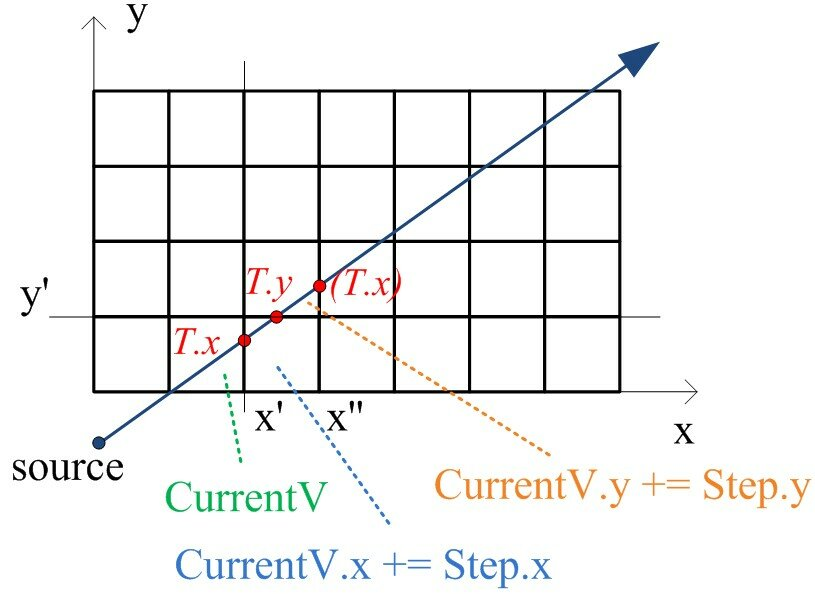
\includegraphics[width=0.8\textwidth]{figures/dda.jpg}}
    \end{center}
    \caption{Illustration of the steps in Digital Differential Analysis (DDA) for ray marching~\cite{Xiao_2019}.}
    \label{fig:dda}
\end{figure}

\subsubsection{Signed Distance Fields (SDF)}
Ray-marching can suffer from difficult shader optimization (if statements nested in for-loops on the GPU), and a large number of steps. Signed Distance Fields use mathematical functions to define the shape and distance to objects; this allows for a key optimization in that the ray can quickly determine the distance to the nearest object and move forward by that amount~\cite{Benton}.

SDFs can therefore be used to represent a voxel grid, using distances to the nearest non-empty voxel. A typical approach for generating an SDF involves iterating through every voxel in the grid and updating it with the distance to the nearest voxel, within a certain distance~\cite{Cummings_2018}. Updating an SDF will therefore also be computationally expensive.

\section{Technical Overview}
This chapter will provide a technical overview of the proposed Signed Distance Field generation algorithm.

To be able to start generating an SDF, a voxel grid is required. The voxel grid will be a 3D occupancy array that will indicate the type of voxel at a given position. The SDF generation algorithm will then require this voxel grid and should iterate over it calculting the distance to the nearest non-empty voxels. Calculating distances for each voxel, to every other voxel in the grid will get exponentially more expensive as the size of the grid grows; it is therefore important to limit the distance to search for neighbours.

The distance to check for neighbours in the SDF generation algorithm will be a key performance optimization as going too far either way could impact generation time, or the ray marching speed due to the number of steps needed to cast the ray through the volume. It will therefore be important to create a simple ray marcher using OpenGL to visualize the SDF.

\section{Workplan}
This section will highlight the key milestones and timeline for the project. Given the complexity of the project, there are also several risks that could impact the success of the project.

\subsection{Timeline}
The project will consist of 4 phases:

\begin{itemize}
    \item \textbf{Phase 1 (Weeks 1-6):} Research and design of Signed Distance Fields, and voxel ray marching techniques.
    \item \textbf{Phase 2 (Weeks 6-12):} Implementation of an SDF generation algorithm for a voxel grid.
    \item \textbf{Phase 3 (Weeks 12-18):} Additional implementation of dynamic updates, and re-generation of the SDF.
    \item \textbf{Phase 4 (Weeks 18-24):} Visualization of results, using a simple ray marcher, to complete dissertation.
\end{itemize}

\subsection{Risks}
Voxel rendering can become a very challenging area to work in as there are many different techniques and systems that can be used and built upon. Creating a fully-fledged voxel render is out-of-scope for this dissertation; however, even so there are some risks:

\begin{itemize}
    \item Inadequate Performance: The generation of the SDF may not meet the aim of supporting 60fps rendering.
    \item Memory Consumption: While optimizing the memory consumption of the SDF, and the raw voxel grid, is out-of-scope; this will somewhat limit the size of voxel grids that can be computed and could affect testing the performance if the memory requirements are so large that only small voxel grids are functional.
    \item Ray Marching: A simple ray-marcher should be implemented to visual the results, and test performance of the generation of the SDF; however, the implementation of the ray marcher may be inefficient and skew results.
    \item OpenGL, Vulkan, GPGPU using CUDA: The choice of the library used to interact with the GPU could affect implementation details and result in differing performance.
\end{itemize}

\bibliographystyle{IEEEtran}
\bibliography{references}

\end{document}
